\documentclass{article}

\usepackage{amsfonts}
\usepackage{amsmath}
\usepackage{amssymb}
\usepackage{amsthm}
\usepackage{caption}
\usepackage{color}
\usepackage{enumerate}
\usepackage{fancyhdr}
\usepackage[margin=1in]{geometry}
\usepackage{hyperref}
\usepackage{graphicx}
\usepackage{latexsym}
\usepackage{listings}
\usepackage{mathrsfs}
\usepackage{natbib}
\usepackage[nottoc]{tocbibind}
\usepackage{setspace}
\usepackage{tikz}
\usepackage{tkz-graph}
\usepackage{url}
\usepackage{topcapt}

\providecommand{\all}{\ \forall \ }
\providecommand{\bs}{\backslash}
\providecommand{\e}{\varepsilon}
\providecommand{\E}{\ \exists \ }
\providecommand{\lm}[2]{\lim_{#1 \rightarrow #2}}
\providecommand{\m}[1]{\mathbb{#1}}
\providecommand{\mc}[1]{\mathcal{#1}}
\providecommand{\nv}{{}^{-1}}
\providecommand{\ov}[1]{\overline{#1}}
\providecommand{\p}{\newpage}
\providecommand{\q}{$\quad$ \newline}
\providecommand{\rt}{\rightarrow}
\providecommand{\Rt}{\Rightarrow}
\providecommand{\vc}[1]{\boldsymbol{#1}}
\providecommand{\wh}[1]{\widehat{#1}}
\providecommand{\thesispaperone}{\cite{thesispaper1}}
\providecommand{\thesispapertwo}{\cite{thesispaper2}}
\providecommand{\thesispaperoneauthor}{\citeauthor{thesispaper1}}
\providecommand{\thesispapertwoauthor}{\citeauthor{thesispaper2}}

\hypersetup{
    colorlinks,
    citecolor=black,
    filecolor=black,
    linkcolor=black,
    urlcolor=blue
}

\pagenumbering{gobble}
\graphicspath{{../fig/}}

\begin{document}

\begin{titlepage}
\pagenumbering{gobble}
\title{A comparison of normalization methods for {\tt fbseq}}
\maketitle

\begin{center}
\vspace{1cm}
\Large
\begin{center}
Will Landau \\ $\quad$ \\
Department of Statistics \\
Iowa State University \\ $\quad$ \\
\end{center}

\vfill
\end{center}
\end{titlepage}

\begin{flushleft}

\section{Introduction}

\paragraph{} In the case study \cite{thesispaper2}, there is a question of how best to compute the normalization factors $h_n$. Currently, we compute them using the method in Section 3.2 (``default"). However, there's also the TMM method (``tmm") \cite{robinson2010scaling}, which is widely-used, and a third option of setting $h_n = 0$ for all $n$ (``zero"). In order to compare these methods in terms of effectiveness, we use several performance metrics described in the case study: mean squared error, receiver operating characteristic (ROC) curves, areas under the ROC curves, calibration curves, and calibration errors. For data, we simulated one dataset with $N = 16$ columns and $G = 30000$ genes for each of the edgeR, model, and simple scenarios described in Section 4.3 of the case study. We analyzed the data with our fully Bayesian approach from Section 3 using the Monte Carlo runtime parameters in Section 3.2. For hardware, we used the Slurm system described at \url{http://it.las.iastate.edu/slurm-simple-linux-utility-resource-management}. The README file at \url{https://github.com/wlandau/normalization/blob/master/README.md} has instructions for reproducing the results below.

\section{Results} \label{sec:results}

\paragraph{} We assessed convergence with Gelman-Rubin potential scale reduction factors on each parameter except for the $\varepsilon_{gn}$'s \cite{bda}. Five of the nine analyses had all Gelman factors below the common tolerance threshold of 1.1. The others had few high Gelman factors, all corresponding to gene-specific parameters. These specific Gelman factors are displayed in Table \ref{tab:gelman}. Any evidence of lack of convergence is weak and unconvincing.

\begin{table}[htbp]
   \centering
   \topcaption{For Section \ref{sec:results}, Gelman-Rubin potential scale reduction factors above 1.1 for the non-$\varepsilon_{gn}$ parameters.} 
   \begin{tabular}{l|l|l|l}
     Dataset & Analysis & Gelman factors & Respective parameters \\ \hline
     edgeR & default & 5.94, 2.33, 1.53, 1.20 & $\beta_{13806, 2}$, $\gamma_{13806}$, $\beta_{13806, 1}$, $\beta_{13806, 3}$ \\
     model & default & 1.50, 1.13 & $\beta_{838, 1}$, $\beta_{15685, 1}$ \\
     model & tmm & 1.26 & $\beta_{838, 1}$ \\
     model & zero & 1.35 & $\beta_{838, 1}$
   \end{tabular}
   \label{tab:gelman}
\end{table}

\paragraph{} Figure \ref{fig:mse} shows mean squared errors (MSE) of the $\beta_{g\ell}$'s for each $\ell$, dataset, and normalization method. MSE appears slightly lower for the TMM method, the edgeR scenario, and $\beta_{g5}$. Otherwise, MSE appear to depend little on the normalization method used.

\begin{figure}[htbp]
   \centering
   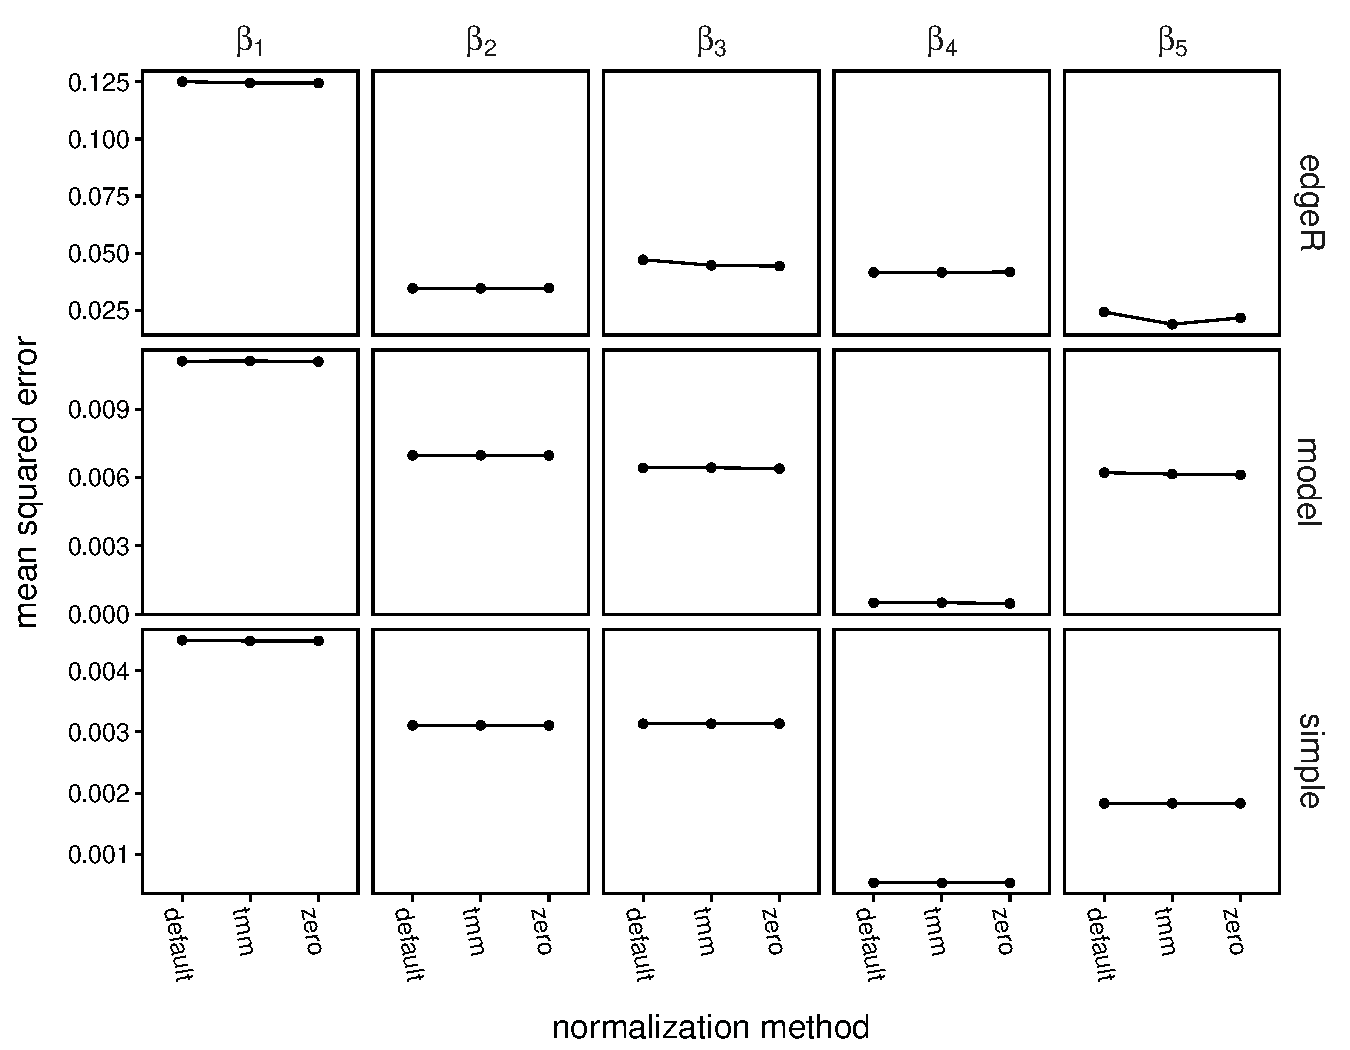
\includegraphics[scale=0.5]{mse}
   \caption{Mean squared errors of the $\beta_{g\ell}$ parameters, shown by simulation (right) and analysis/normalization (bottom) methods.}
   \label{fig:mse}
\end{figure}

\paragraph{} Figure \ref{fig:roc} shows receiver operating characteristic (ROC) curves for each dataset, analysis, and mode of heterosis. From this figure, differences in performance among the normalization methods appear extremely small and possibly insignificant. The biggest differences are seen for the ``high H21" and ``high mean" modes of heterosis, which favor the default method the best and the ``zero" method the worst. 

\begin{figure}[htbp]
   \centering
   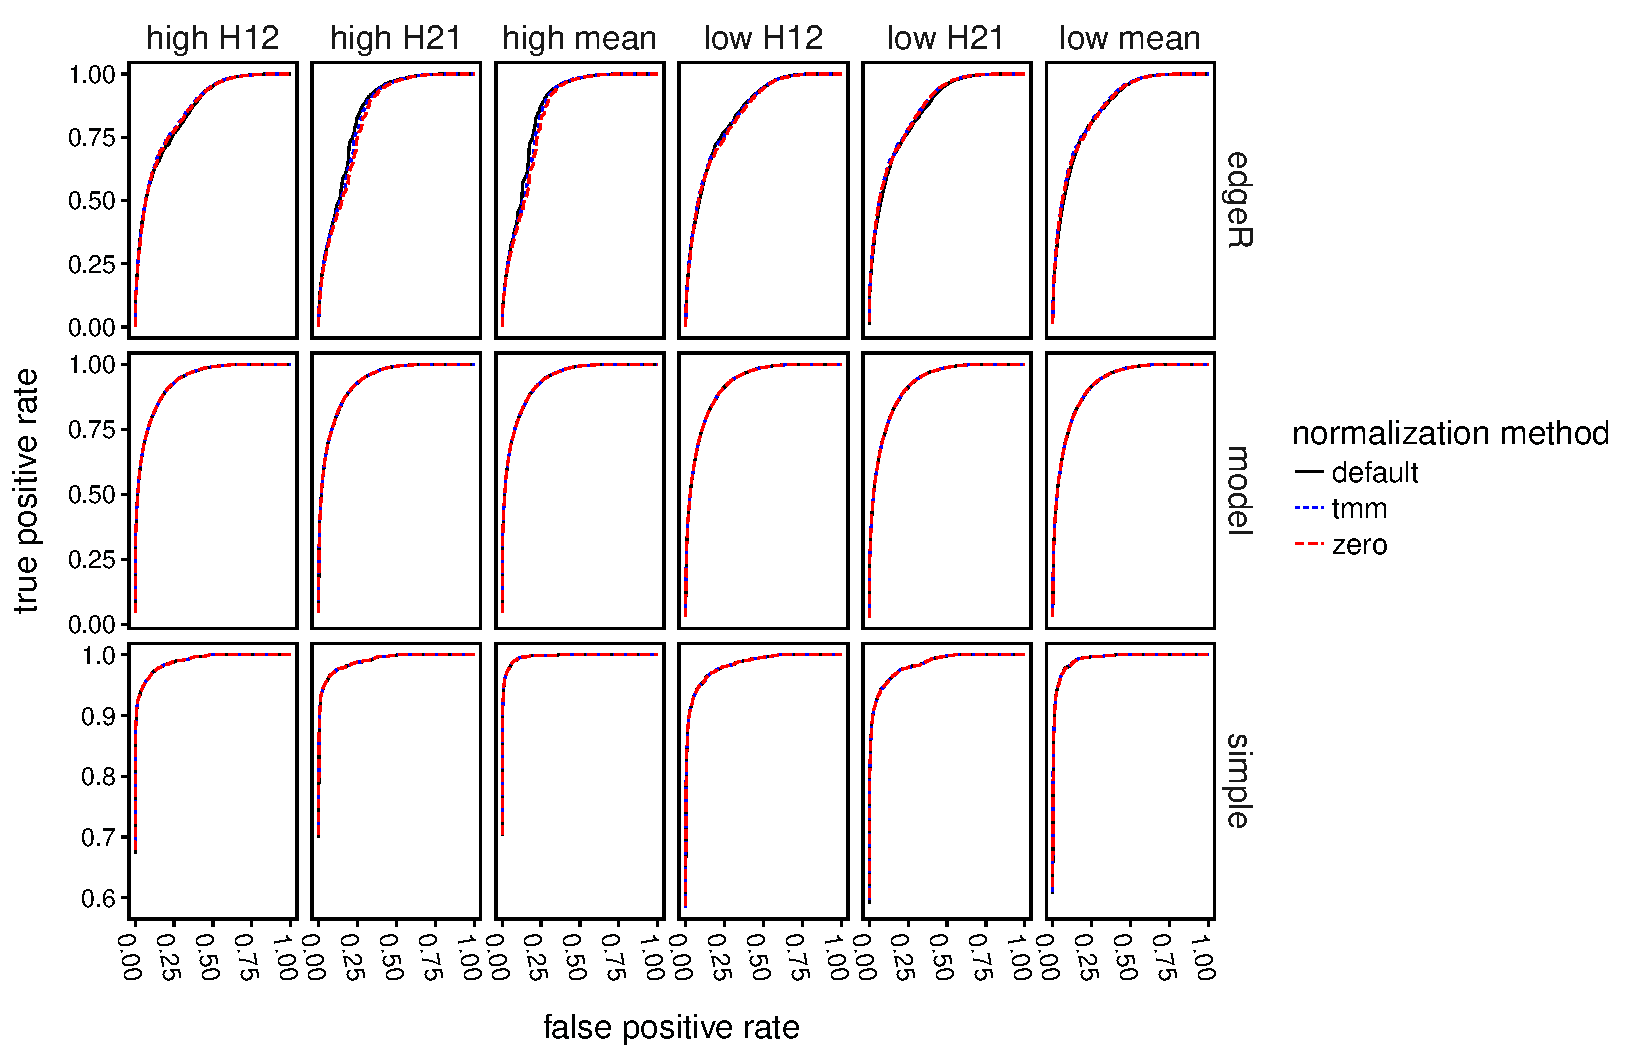
\includegraphics[scale=0.5]{roc}
   \caption{Receiver operating characteristic (ROC) of heterosis gene detection. The type of heterosis, as explained in the case study \cite{thesispaper2}, is indicated at the top, and the dataset is indicated on the right.}
   \label{fig:roc}
\end{figure}

\paragraph{} Figure \ref{fig:auc} shows the areas under the ROC curves (AUC) in Figure \ref{fig:roc}. Subtle differences in performance are magnified here. Apparently, the default normalization method outperforms TMM and ``zero" for the ``high H21" and ``high mean" modes of heterosis in the edgeR dataset. Everywhere else in the edgeR dataset, the TMM method does at least as well as the default and ``zero" methods, outperforming them except for the ``low H12" mode of heterosis. Differences in AUC for the model and simple datasets appear extremely small to insignificant.

\begin{figure}[htbp]
   \centering
   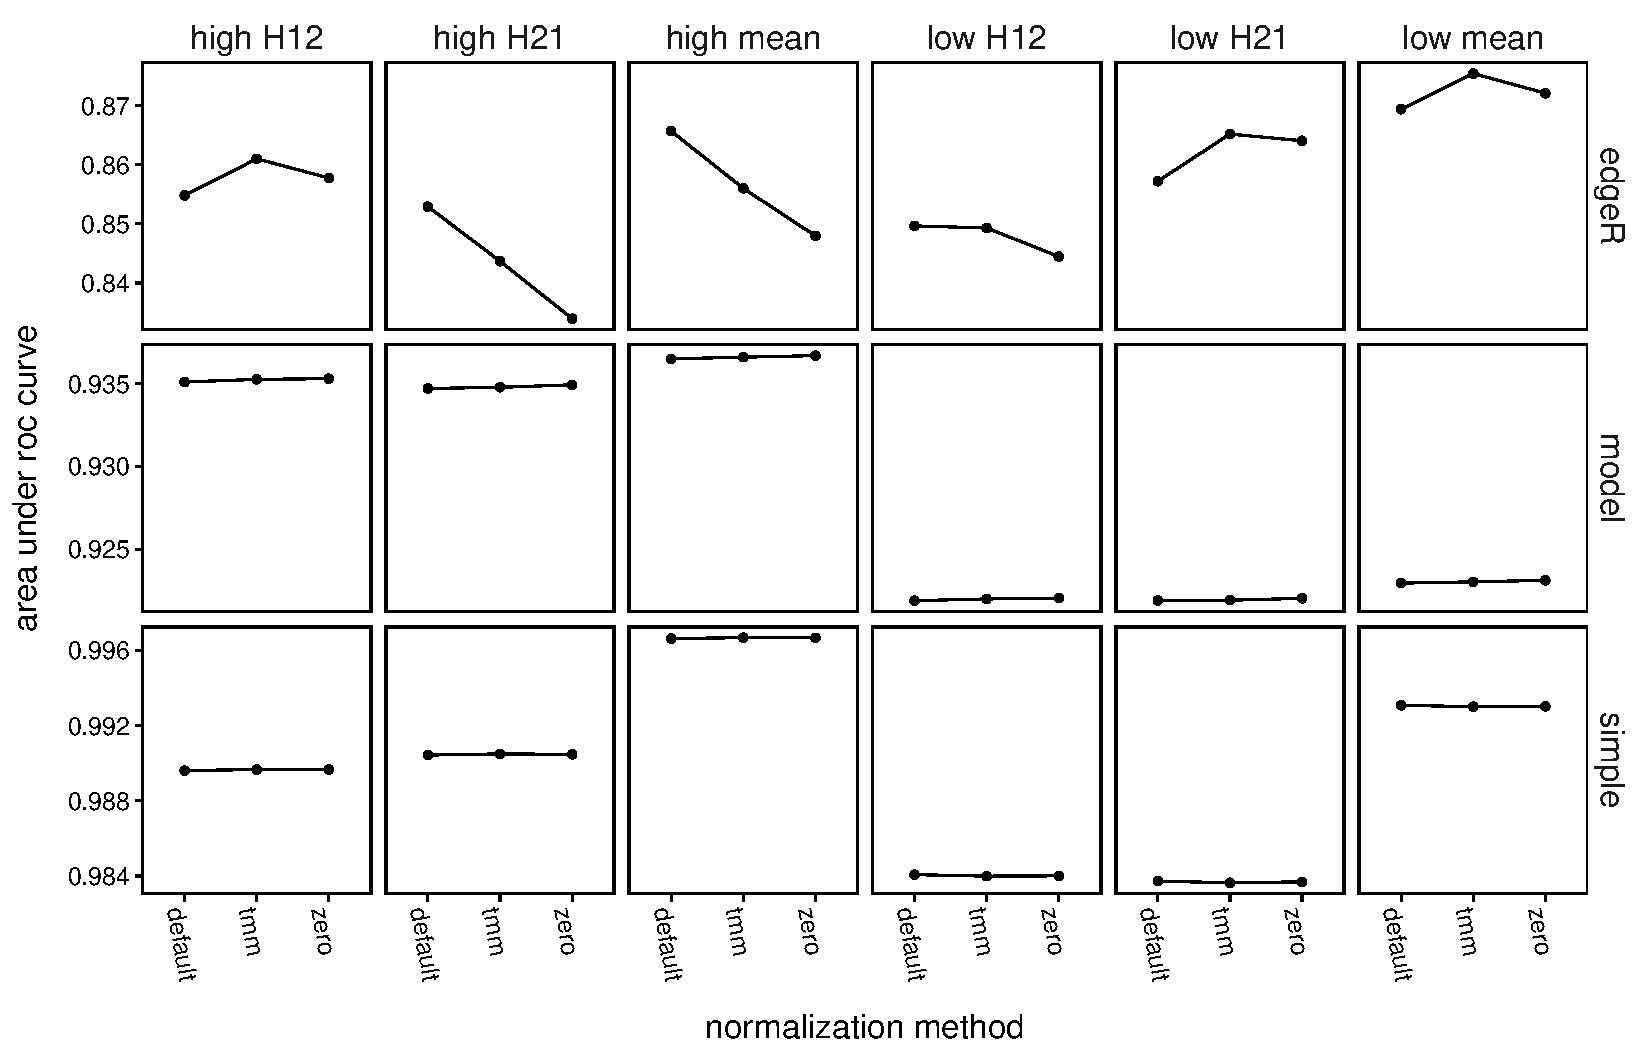
\includegraphics[scale=0.5]{auc}
   \caption{Areas under the ROC curves in Figure \ref{fig:roc}.}
   \label{fig:auc}
\end{figure}

\paragraph{} Figure \ref{fig:calibration} shows calibration curves. Differences in calibration are extremely small for the model and simple scenarios. For the edgeR scenario, differences are more pronounced. The default method appears to perform uniformly worse than the TMM method for low-parent heterosis, but better than TMM for high-parent heterosis when probabilities exceed 0.5. 

\begin{figure}[htbp]
   \centering
   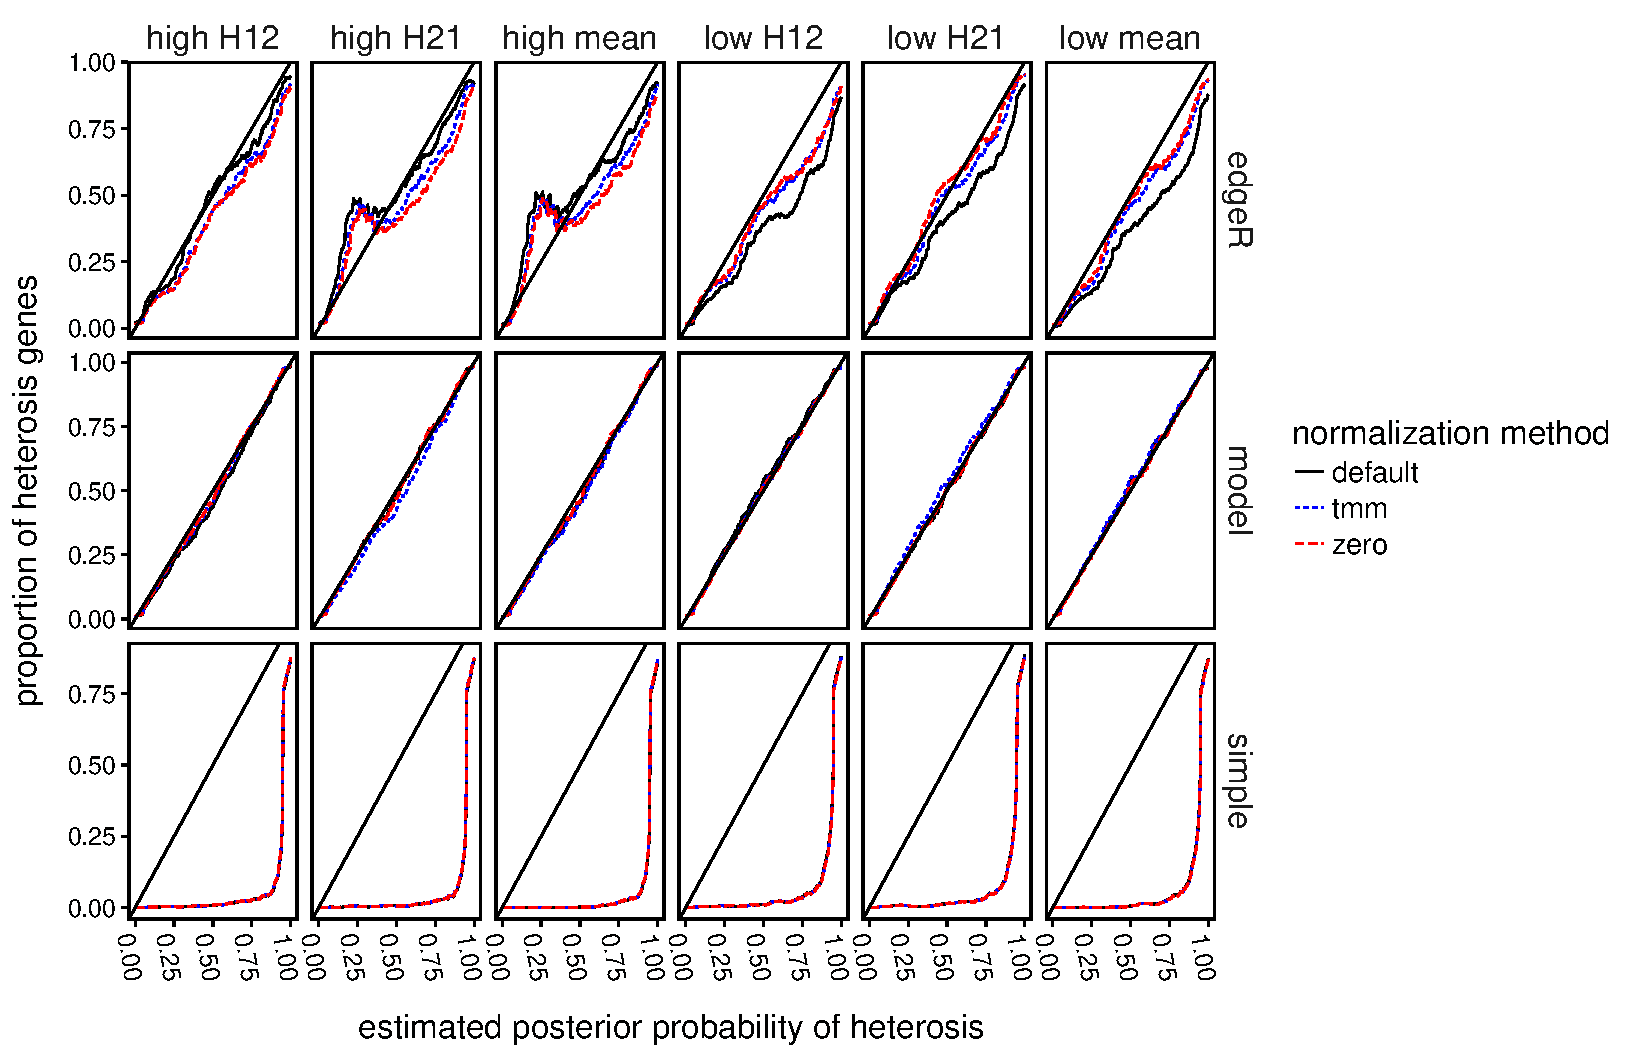
\includegraphics[scale=0.5]{calibration}
   \caption{calibration}
   \label{fig:calibration}
\end{figure}

\paragraph{} Figure \ref{fig:calibrationerror} shows the calibration errors taken from the calibration curves in Figure \ref{fig:calibration}, magnifying the overall differences in the calibration of posterior probabilities of heterosis. Differences among normalization methods within the simple dataset appear negligibly small. For the ``model" dataset, the TMM method appears to perform mostly worst, but from a glance at the uniformly excellent calibration curves in Figure \ref{fig:calibration} tells us that this performance loss is extremely small to insignificant. For the edgeR scenario, where differences in calibration are more significant, the rankings are clear. For high-parent heterosis, the ``zero" method is the best and the default method is the second-best. For low-parent heterosis, this ranking completely reverses. 

\begin{figure}[htbp]
   \centering
   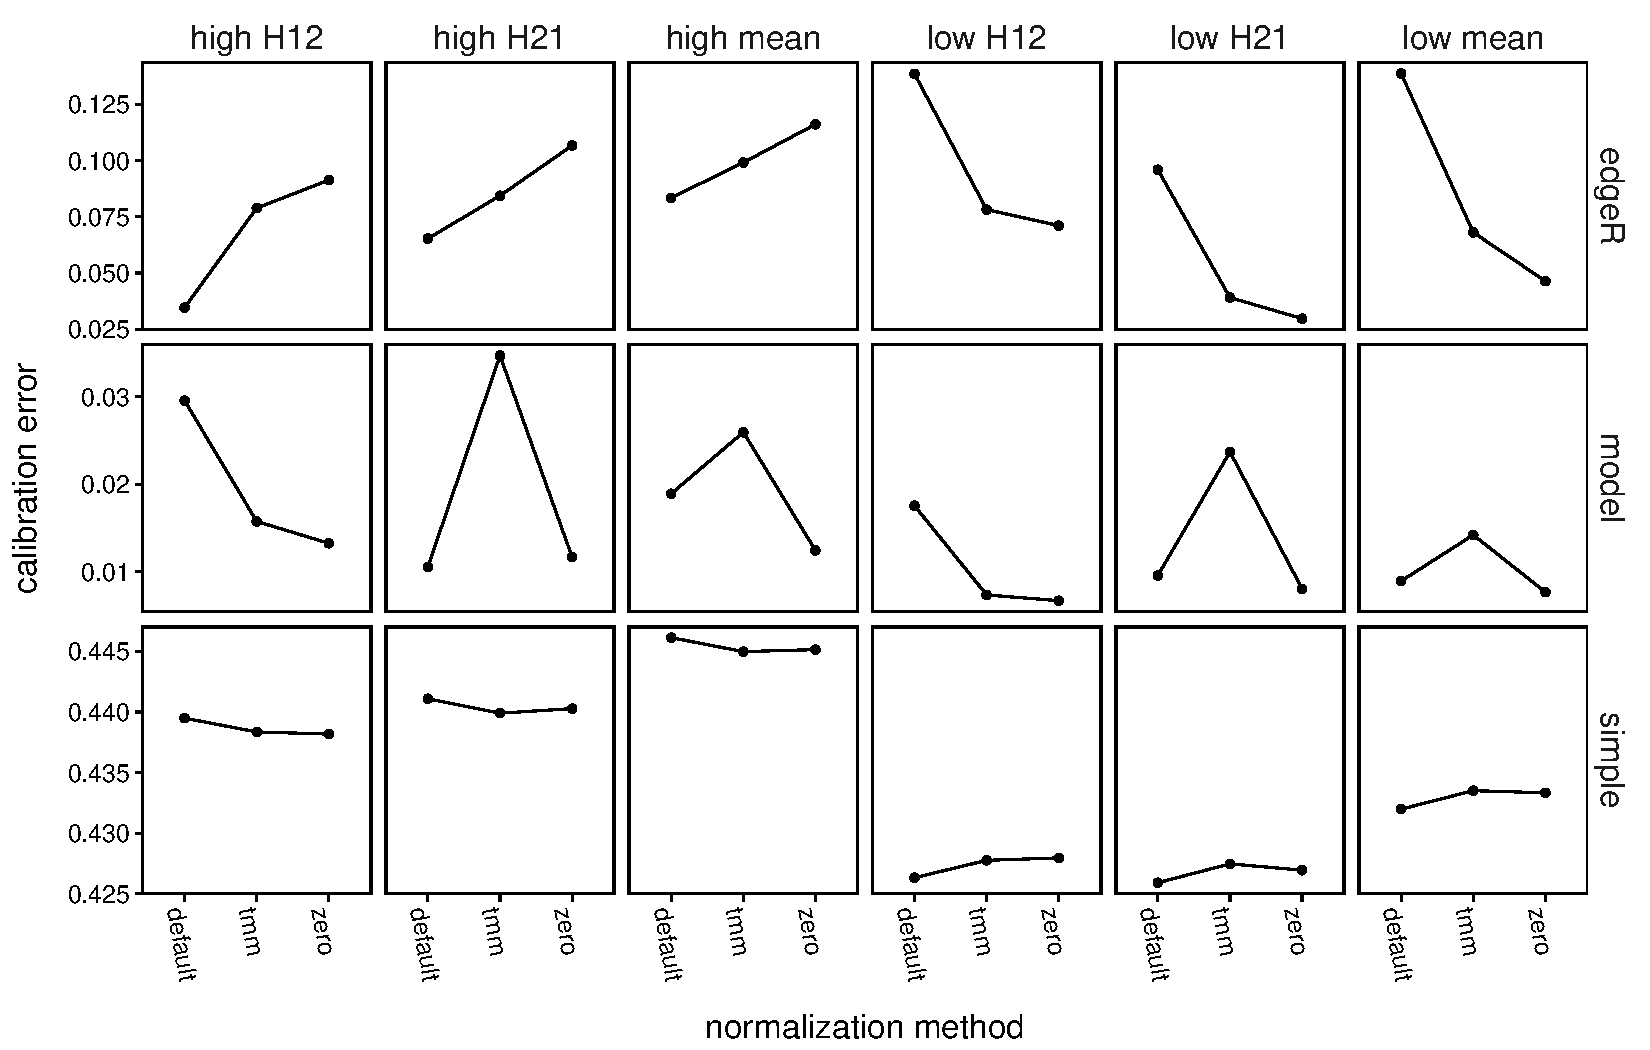
\includegraphics[scale=0.5]{calibration_error}
   \caption{Calibration errors taken from the calibration curves in Figure \ref{fig:calibration}.}
   \label{fig:calibrationerror}
\end{figure}

\section{Conclusion}

For our three simulated datasets, with respect to MSE and ROC curves, the choice of normalization method for the $h_n$'s appears inconsequential. Normalization does start to matter once we consider calibration, but there, the performance ranking for high-parent heterosis is the reverse of that of low-parent heterosis. So far, unless we exclude high-parent heterosis, there is no reason to prefer TMM over our default normalization method.

\end{flushleft}
\bibliographystyle{plain}
\bibliography{report}
\end{document}